\chapter{Methodologies}
\graphicspath{{Chapter3/Figs/}{Chapter3/Figs/}}

This chapter describes the project-related academic methodologies in the given circumstances of the author and the planned approach to achieve the thesis's goals and objectives. The reader is introduced to the rationale for the intended workflows, hardware, and software tools.

\section{Derivation of the case study}
\label{chapter3-derivation-of-the-case-study}

In October 2021, the author began working as a cloud software engineer at IDUN Technologies, an ETH spin-off startup in Zürich, to further develop their existing software products. IDUN had already created a PoC software system that included a web-based single-page application (SPA) hosted on AWS Amplify, a backend-as-a-service product aiming to simplify the deployment of backends for mobile and web apps. IDUN's in-ear sensor sent EEG data to a physical network bridge via Bluetooth and then to the cloud via the internet. The raw EEG data\footnote{Raw EEG data refers to data measured by the in-ear sensor without any additional processing.} was saved and made available for download in various file formats.

\begin{figure}[!ht]
  \centering
  
\includegraphics[width=\linewidth]{raw-filtered-data.png}
  \caption{Difference between raw and filtered data from IDUN's product.}
  \label{fig:raw-filtered-eeg}
\end{figure}

In addition to raw data, the IDUN SPA provided processed data, such as, e.g. filtered data, which included low-pass and high-pass filtering of EEG data as shown on \autoref{fig:raw-filtered-eeg}. This processed EEG data was then saved alongside the raw version on the cloud.

The EEG data could also be visualised in near-real-time on the SPA as a time-series x- and y-axis plot. Additionally, users could control the device by sending start and stop commands to the hardware components. The PoC system, whose architecture is shown on \autoref{fig:idun-amplify}, was in a relatively unstable state and had various error sources that made it impossible to reliably record EEG data for more than a few minutes, making the product unusable for existing customers or a mass-market launch. While working on the system, the author encountered various technological bugs and flaws as described in \autoref{appendix2-flaws-and-bugs-previous-system}.

\begin{figure}[!ht]
  \centering
  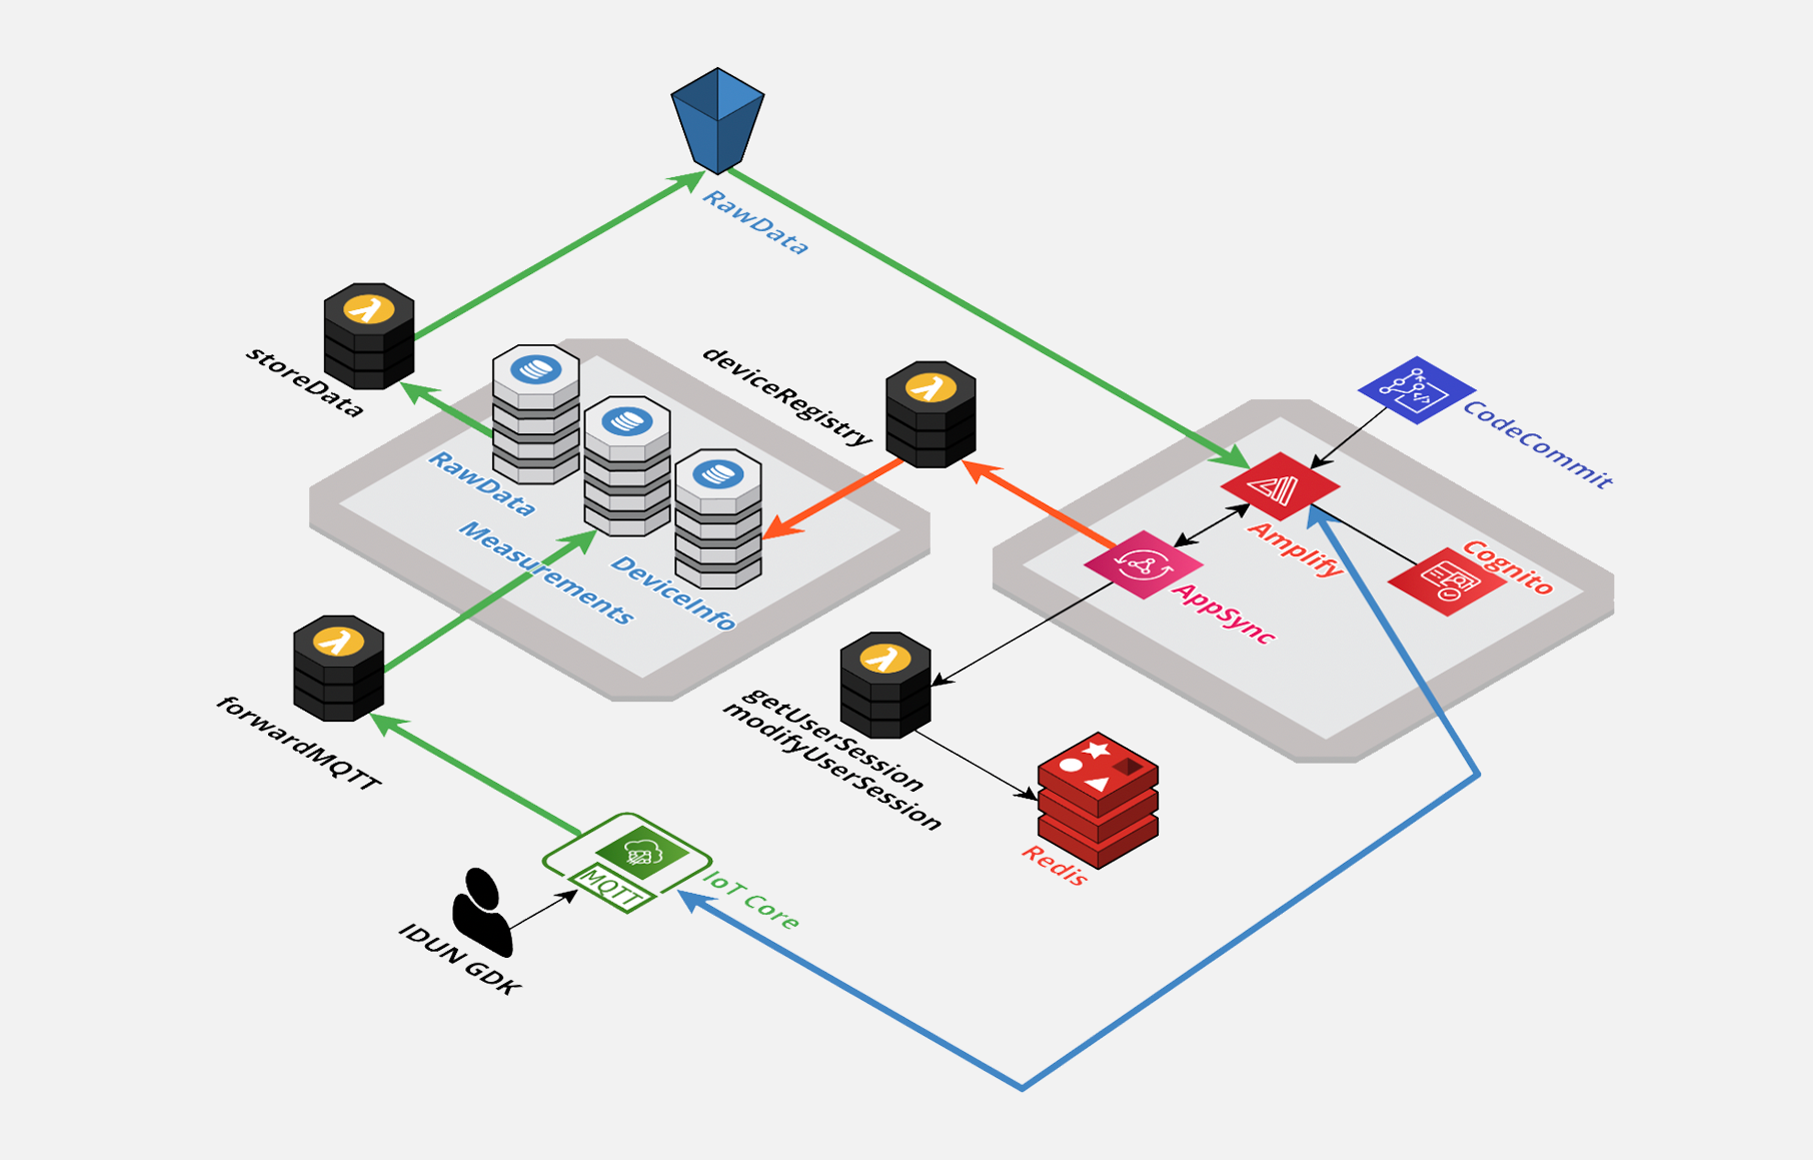
\includegraphics[width=\linewidth]{idun-amplify.png}
  \caption{IDUN's software architecture at the end of 2021.}
  \label{fig:idun-amplify}
\end{figure}

Due to growing challenges with the existing software system and an ever-increasing technical debt as a result of the software not being test-driven or developed without clean code quality standards, resulting in bugs and quirks that are difficult to track down, the author proposed to halt the implementation of new features and restructure the system from the ground up using a more software engineering-oriented approach. The company's management approved the request for this redevelopment in early December 2021. At the time, the author was already working on his original Bachelor project, which focused on a EEG-controlled multiplayer game, assuming that IDUN's software system would be stable by the time the Bachelor project began. The original Bachelor project's focus was officially changed at the end of 2021 to create a thesis on the redevelopment of IDUN's cloud software.

\section{Case study}
\label{chapter3-case-study}

As previously mentioned, IDUN Technologies is a full-stack company which produces in-ear EEG sensors in the form of earphones. Their vision is to sell their hardware and license a software product coupled with the hardware called Neuro-Intelligence Platform (NIP), as shown on \autoref{fig:idun-nip}.

\begin{figure}[!ht]
  \centering
  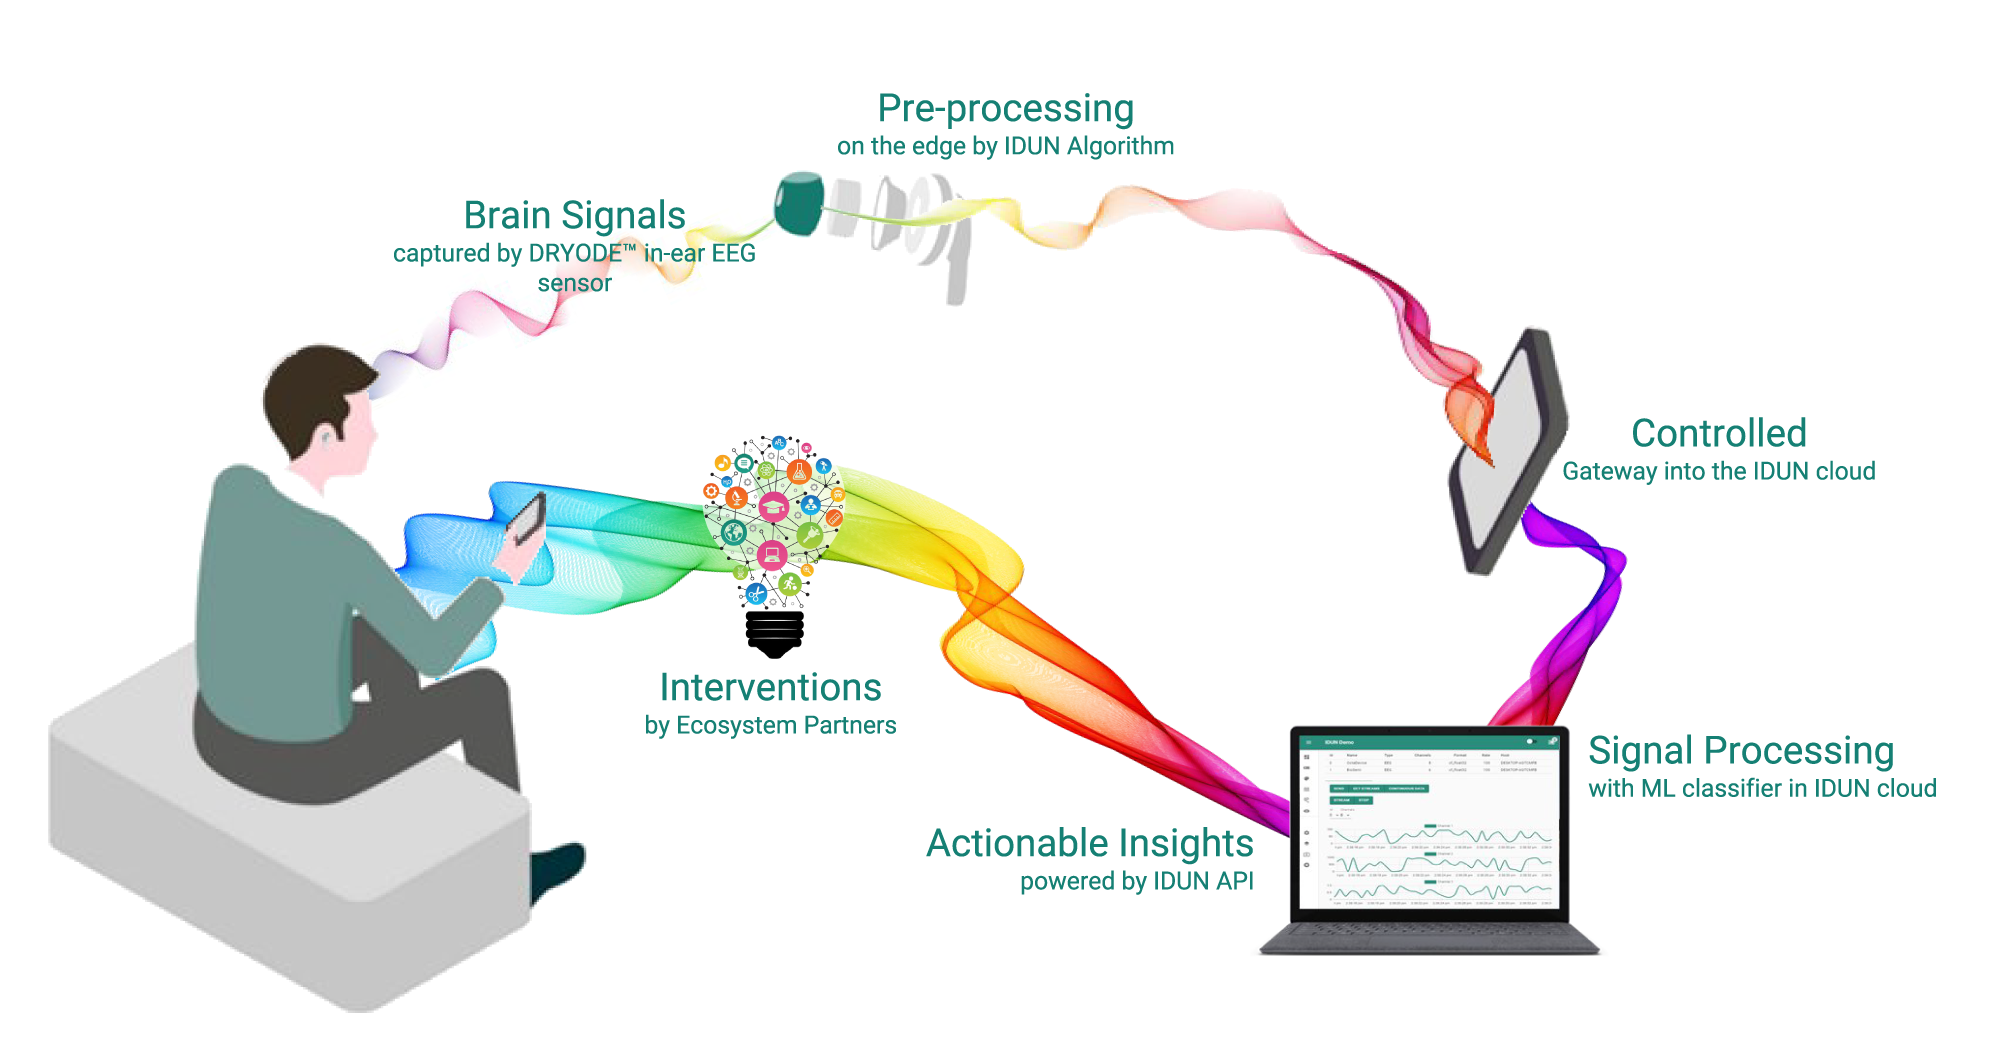
\includegraphics[width=\linewidth]{idun-nip.png}
  \caption[IDUN's vision of a closed neurofeedback loop ]{IDUN's vision of a closed neurofeedback loop \citep{idun_guardian_nodate}.}
  \label{fig:idun-nip}
\end{figure}

The mission is essential that an unobtrusive BCI device, such as an in-ear headset, can be worn for the majority of the day while measuring neural data that is sent in real-time to the cloud to process and classify actionable insights that other developers can use to build their interventions (e.g., apps, websites, and games) on top of it to promote mental health and well-being. Furthermore, the aspect of longitudinal data is essential, implying that it could be advantageous to store neural data over a long period and run classifiers on it from time to time to understand one's brain better which is one of the possible solutions described for the lack of data challenge in \autoref{chapter2-lack-of-data}.

Moreover, it is essential to select an appropriate research method to develop a system that would fulfil the company's mission and vision. The author chose a case study because it is an effective method for dealing with unusual and atypical cases while providing new and unexpected perspectives in certain situations such as in a deep-tech startup like IDUN.

\section{Procedure}
\label{chapter3-procedure}

This section describes the planned procedure for conducting a case study-based research methodology to develop the proposed N/CI at IDUN Technologies as part of their NIP.

\subsection{Project stages}
\label{chapter3-project-stages}

The goal was to conduct qualitative research and examine the use case from various perspectives. In addition, two other methodologies were used in the case study: 1. Expert interviews, which entails locating experts on topics such as cloud or BCI and asking them questions that will assist in answering implementation questions, and 2. group discussions, which aim at learning about people's attitudes and opinions about related topics.

\begin{figure}[!ht]
  \centering
  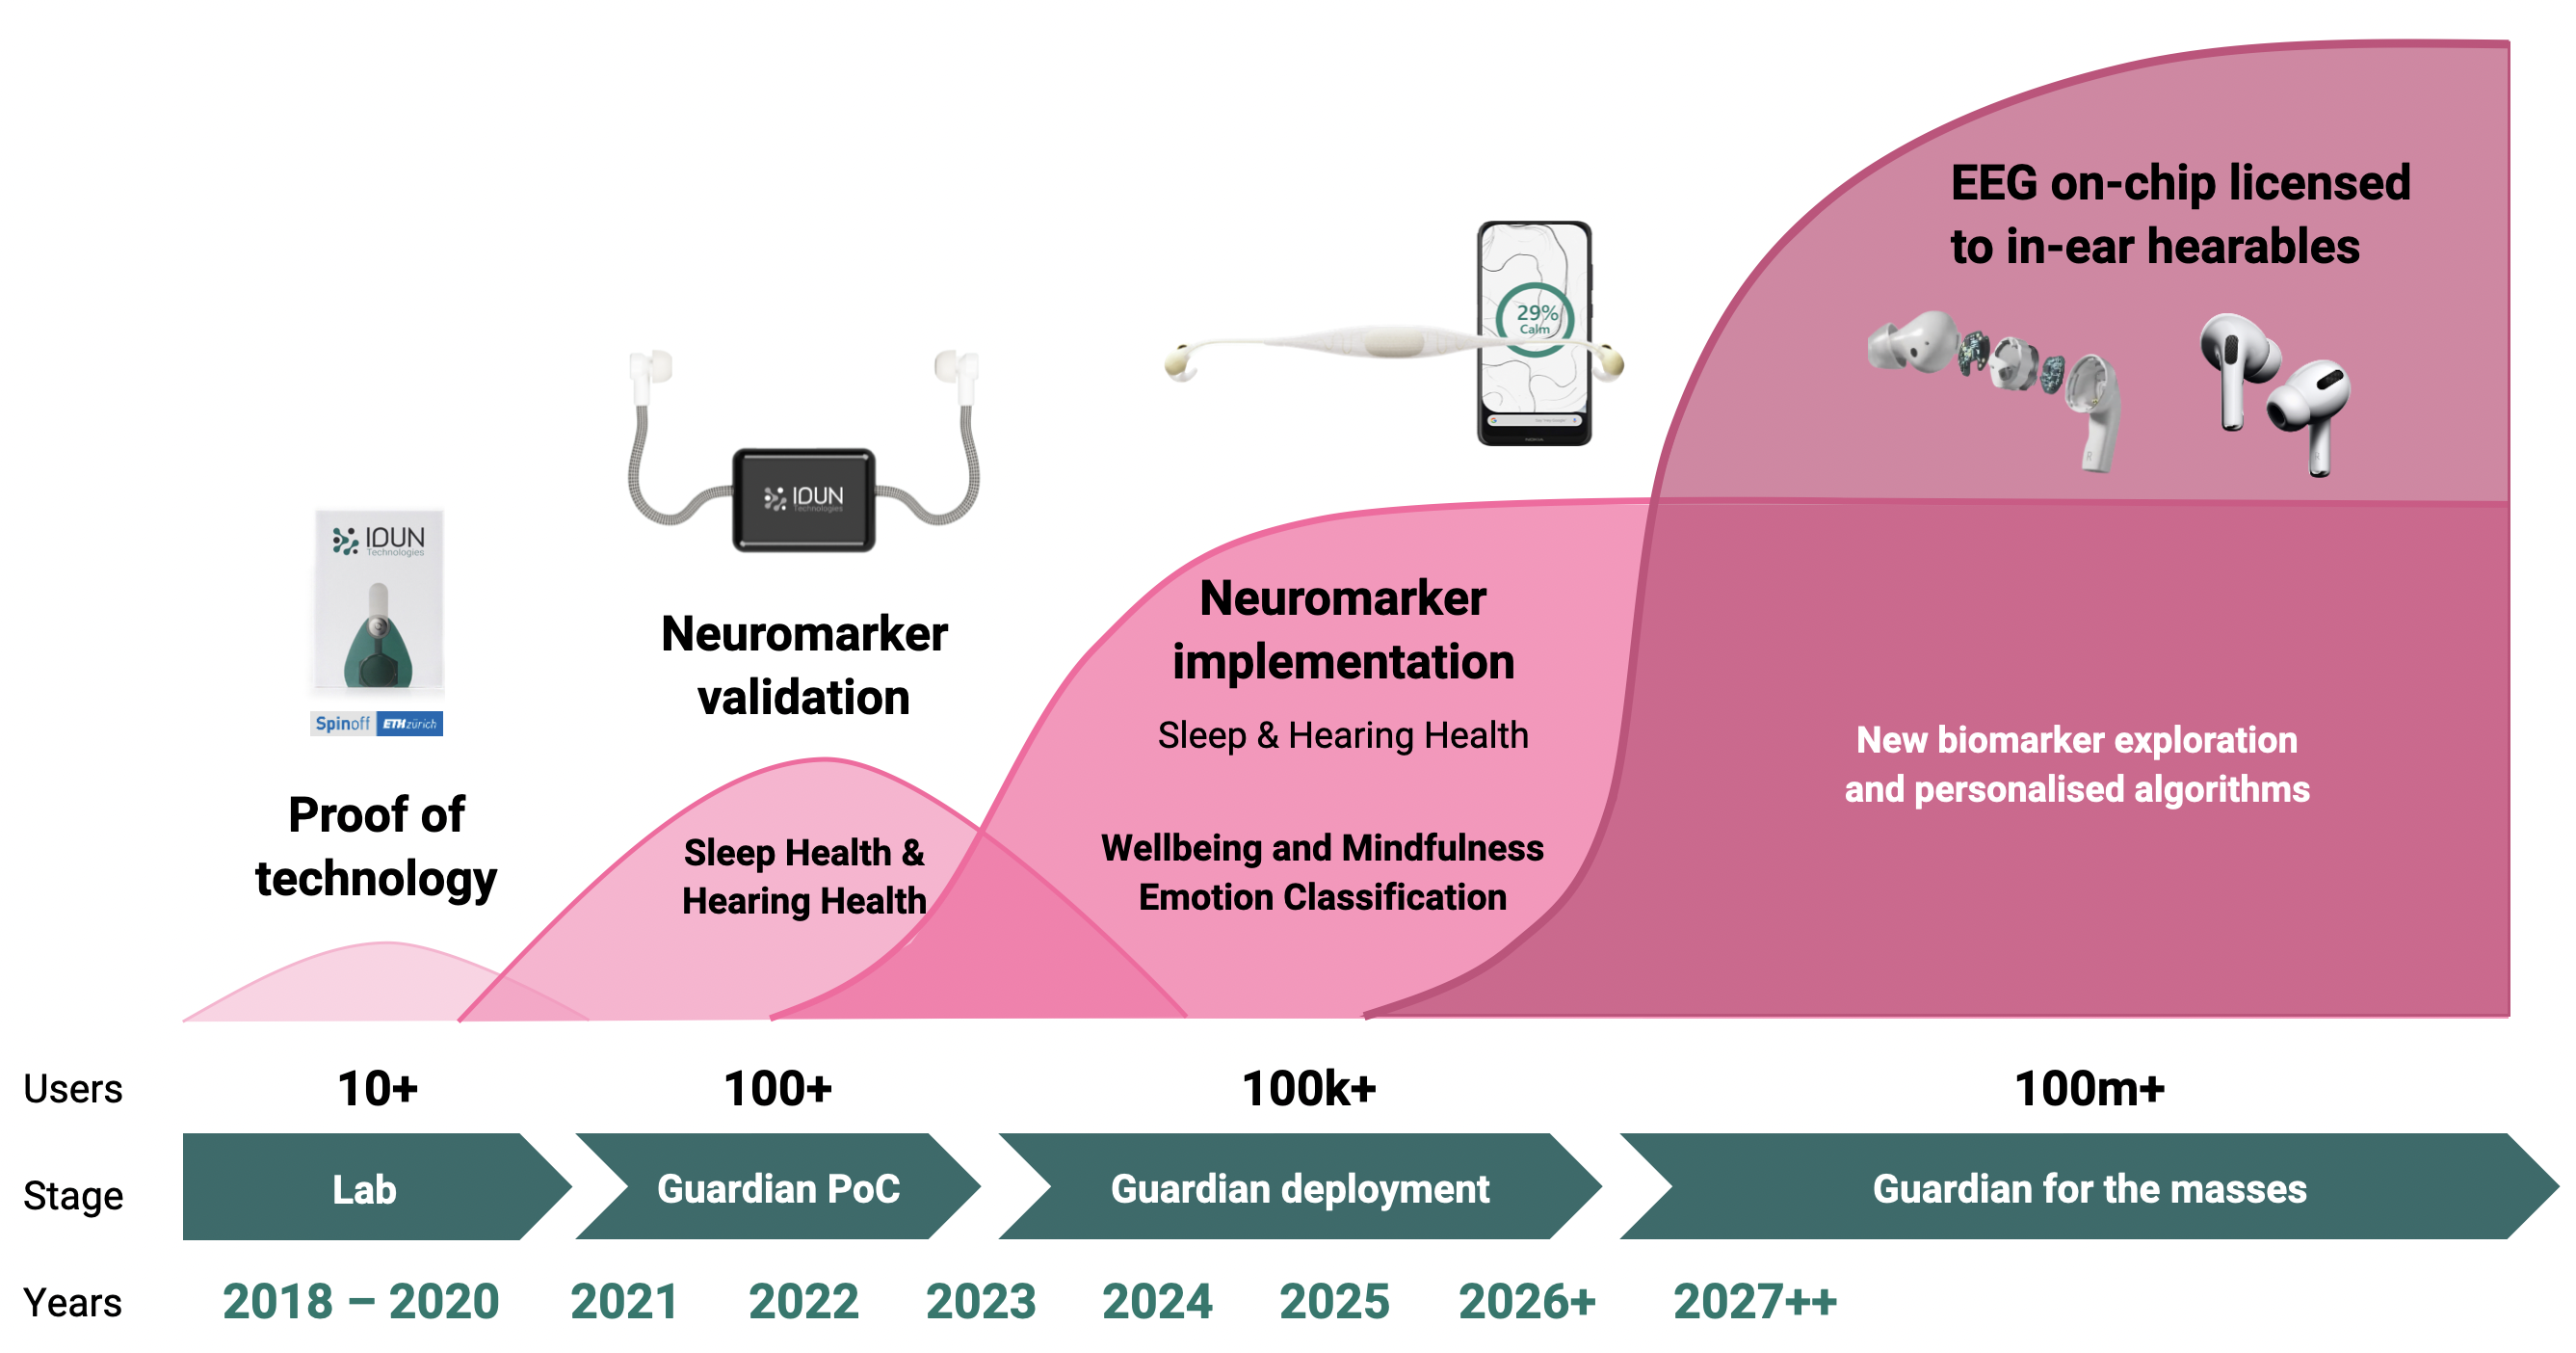
\includegraphics[width=\linewidth]{idun-timeline.png}
  \caption[IDUN's plan to achieve their goals]{IDUN's plan to achieve their goals \citep{idun_guardian_nodate}.}
  \label{fig:idun-timeline}
\end{figure}

Before defining the project stages, it is essential to look at the timing of IDUN's roadmap as shown on \autoref{fig:idun-timeline}. There are three essential pieces of information: The stage in which the technology resides, the estimated user base size, and the time frames of these stages that want to be achieved. The author was working towards a version starting to be released in 2023, ergo working on the N/CI placed in the Guardian deployment phase. As the company is still implementing the first neuromarkers into the product and is focusing on two use cases, namely sleep and hearing health, due to the size of the team and the mass production of hardware and sensors, the sales team is targeting the sale of devices to about 100'000 people. Another constraint is the deadline of the bachelor's thesis of the author, which is set on the 5th of August 2022. User size, company stages and the deadline for the thesis are important context information for defining the project stages for this use case. Following on \autoref{tab:project-stages} are the proposed project stages to execute the case study:

\begin{table}[!ht]
  \centering
  \resizebox{\textwidth}{!}{%
    \begin{tabular}{
        >{\columncolor[HTML]{FFFFFF}}l l}
      \cellcolor[HTML]{000000}{\color[HTML]{FFFFFF} Project stage}                                                                                             &
      \cellcolor[HTML]{000000}{\color[HTML]{FFFFFF} Description}                                                                                                                                                                                                                                                                                                                                                                                                                                                                                                                                                                                                   \\ \hline
      \multicolumn{1}{|l|}{\cellcolor[HTML]{FFFFFF}\textbf{\begin{tabular}[c]{@{}l@{}}1.1 Define key technical\\ requirements and\\ constraints\end{tabular}}} &
      \multicolumn{1}{l|}{\begin{tabular}[c]{@{}l@{}}Based on the internal hardware, the neuroscience and data science departments and the IDUN mission\\ and roadmap, the author needs to define the purely technical requirements and constraints. Some\\ constraints are e.g. hiring of advisors, time limits and risks due to investment rounds. Some purely\\ technical requirements come from e.g. the firmware team or the material scientists, such as maximum\\ latency or the data structure of the digitalised and amplified EEG.\end{tabular}}                                                                                                         \\ \hline
      \multicolumn{1}{|l|}{\cellcolor[HTML]{FFFFFF}\textbf{\begin{tabular}[c]{@{}l@{}}1.2 Extensive literature\\ research\end{tabular}}}                       &
      \multicolumn{1}{l|}{\begin{tabular}[c]{@{}l@{}}Already since the beginning of the original bachelor thesis, the author started to do literature research in\\ the field of BCI, which is very helpful for the new focus. Further literature review now includes\\ books on data intensive applications and cloud, articles and research papers.\end{tabular}}                                                                                                                                                                                                                                                                                                \\ \hline
      \multicolumn{1}{|l|}{\cellcolor[HTML]{FFFFFF}\textbf{\begin{tabular}[c]{@{}l@{}}2.1 External user\\ interviews\end{tabular}}}                            &
      \multicolumn{1}{l|}{\begin{tabular}[c]{@{}l@{}}Defining users personas with IDUN's product manager, application engineer and sales team, finding\\ real people to represent these personas, preparing an external interview framework and questions,\\ gathering as many insights as possible.\end{tabular}}                                                                                                                                                                                                                                                                                                                                                 \\ \hline
      \multicolumn{1}{|l|}{\cellcolor[HTML]{FFFFFF}\textbf{\begin{tabular}[c]{@{}l@{}}2.2 Creative workshop and\\ prototyping\end{tabular}}}                   &
      \multicolumn{1}{l|}{\begin{tabular}[c]{@{}l@{}}Based on the insights from the user interviews, conduct a creative workshop with IDUN's product\\ manager and application engineer. The results are design artefacts such as wireframes, user flows,\\ interactive prototypes and architecture diagrams which are essential for internal group discussions.\end{tabular}}                                                                                                                                                                                                                                                                                     \\ \hline
      \multicolumn{1}{|l|}{\cellcolor[HTML]{FFFFFF}\textbf{\begin{tabular}[c]{@{}l@{}}3.1 Internal group\\ discussions\end{tabular}}}                          &
      \multicolumn{1}{l|}{\begin{tabular}[c]{@{}l@{}}The design artefacts are used for an internal validation with the department heads. Several group\\ discussions are held with each department, ranging from materials science to business development.\\ Based on the group discussions, the artefacts are adapted and improved.\end{tabular}}                                                                                                                                                                                                                                                                                                                \\ \hline
      \multicolumn{1}{|l|}{\cellcolor[HTML]{FFFFFF}\textbf{3.2 Expert interviews}}                                                                             &
      \multicolumn{1}{l|}{\begin{tabular}[c]{@{}l@{}}Define experts in different areas of BCI, cloud and EEG, and neuroethics. Create a framework for\\ expert interviews and questions that are still unclear or open based on the design artefacts. Conduct\\ expert interviews and gather as many insights as possible to adapt and improve the design artefacts.\end{tabular}}                                                                                                                                                                                                                                                                                 \\ \hline
      \multicolumn{1}{|l|}{\cellcolor[HTML]{FFFFFF}\textbf{4. Start bootstrapping}}                                                                            &
      \multicolumn{1}{l|}{\begin{tabular}[c]{@{}l@{}}While the design process is still ongoing, you can already start implementing the most important\\ technical requirements, with anything that is a flexible bootstrapping of internal development\\ processes to ensure quality assurance, for example, not being tied to the other phases.\end{tabular}}                                                                                                                                                                                                                                                                                                     \\ \hline
      \multicolumn{1}{|l|}{\cellcolor[HTML]{FFFFFF}\textbf{\begin{tabular}[c]{@{}l@{}}5. Iterative and agile\\ implementation via\\ Scrum\end{tabular}}}       &
      \multicolumn{1}{l|}{\begin{tabular}[c]{@{}l@{}}IDUN works with Scrum, for this the author has introduced Scrum in the research and development\\ department. Scrum at IDUN has three-week sprints and there are ten sprints from January 2022 to the\\ end of July 2022 that can be used to go through the design process and implement the designs. In the\\ process, there are several iterative processes to validate and test the increments of the system based on\\ insights from the implementation, ongoing literature research, insights from other departments or the\\ design process (i.e. user interviews) that is still ongoing.\end{tabular}} \\ \hline
    \end{tabular}%
  }
  \vspace{10pt}
  \caption{Project stages of this thesis.}
  \vspace{-5pt}
  \label{tab:project-stages}
\end{table}

Number 1.1 is crucial before starting anything else. Number 1.2 is continuously in progress. Numbers 2.1 to 3.2 take place simultaneously while number 4 is ongoing\footnote{Number 4 refers to bootstrapping, which usually refers to the practice of setting up development environments that include, e.g. initial Git repositories, folder structures and creating accounts on cloud providers.}. As soon as numbers 3.2 and 4 are completed, number 5 can be started.

\subsection{Group discussions}
\label{chapter3-group-discussions}

According to the author, it is critical to conduct user interviews with external people. Consequently, this informs the development of a deep-tech focused product in such a way that one does not require to have extensive company-specific knowledge. Based on the user interviews, the goal is to create design artefacts in the design tool Figma for GUI-related topics as well as in the whiteboard collaboration tool Miro for architecture-related topics. These design artefacts are utilised to communicate the outputs of design process to IDUN's internal staff based on the findings from the external user interviews. The ideas and findings should be presented and validated concerning IDUN staff's understanding and product perceptions via internal group discussions. Because the development of a complete neurotechnology product involves many disciplines ranging from physics to machine learning, the company must have a shared understanding of what the software component of the NIP, ergo the N/CI, will look like and what for functionalities it will have.

\subsection{Expert interviews}
\label{chapter3-expert-interviews}

It is critical to consult experts after the external and internal validation and design process and its iteration through group discussions. In the author's experience, it is difficult to, e.g. engage consultants at an early stage of the process without knowing what one wants to build because advisors, e.g. from a consultancy firm, tend to push for commercially oriented ideas to generate their revenue rather than thinking about the project's long-term success. Experts are chosen based on the author's experience and the experience of other IDUN Technologies employees, such as data scientists and neuroscientists. According to a previous blog post by the author, the importance of ethics in the field of BCI is critical \citep{burger_influence_2021}. As a result, it is crucial to include neuroethics experts in the plans and ideas for IDUN's N/CI as well.

\section{Software and tools}
\label{chapter3-software-and-tools}

There is a great amount of software and tools that can be used to construct a comprehensive software system, such as IDUN's N/CI. The author had some leeway in deciding which software and tools (i.e. libraries and frameworks) to use. Nonetheless, some software and tool limitations should be considered diving into the implementation:

\begin{itemize}
  \item IDUN has received a large number of credits from Amazon for its AWS account, which should therefore be used to avoid creating redundant costs when using another cloud provider.
  \item The Python ecosystem has strong roots among engineers and researchers at IDUN, which should be taken into account. An example of this are the Python packages SciPy or MNE for processing and visualising EEG data, which do not exist in any other language.
  \item The author needs to familiarise himself with the software and tools required to build IDUN's N/CI. For example, the AWS cloud would be an example where the author has to transfer his knowledge from the Google Cloud Platform (GCP) experience and understand different ways of implementing certain cloud features in AWS.
  \item Any new tool that is not open source and free to use should be carefully considered in terms of future maintainability, security and learning effort.
  \item Wherever possible, redundancy in the workload should be avoided, as a venture capital-funded startup like IDUN has a particular runway time that describes the company's remaining time before it runs out of cash. Spending, e.g. an entire sprint working on something that is then thrown away, can be business-critical, so every software and tool decision is carefully weighed.
\end{itemize}

\section{Checkpoints for progress}
\label{chapter3-checkpoints-for-progress}

Progress is reviewed at the end of each three-week sprint. IDUN's entire research and development team and stakeholders, such as C-level management, attend the review events. Each department asks questions about the author's progress and findings. The planning for the upcoming sprint will take place based on the topics discussed in the reviews. Asana, a project management tool, mirrors the overall product backlog and the personal backlog of the author's bachelor project and tracks progress in terms of story points and remaining epics in its dashboard. In addition to Asana, documentation of all project stages will be documented in Notion. Screenshots of the mentioned documents will be attached in \autoref{appendix7-other-documents}.

Before moving on to the next chapter, the author would like to highlight an important point: The quality of the proposed project stages is an essential part, made even more crucial when one considers the extensive list of flaws in the current IDUN software system summarised in \autoref{appendix2-flaws-and-bugs-previous-system}. This can only be avoided by implementing extensive quality assurance measures (i.e. unit tests and automated continuous integration pipelines) during the bootstrapping project stage. To quote Robert C. Martin from his Clean Architecture book: “The only way to go fast, is to go well” \citep{martin_clean_2018}.

\nomenclature[nip]{NIP}{Neuro-Intelligence Platform}
\nomenclature[spa]{SPA}{Single-page application}
\nomenclature[mqtt]{MQTT}{Messaging and queuing middleware telemetry transport}
